\documentclass[11pt,a4paper]{article}

\usepackage[utf8]{inputenc}
\usepackage[T1]{fontenc}
\usepackage[spanish,es-noindentfirst]{babel}
\usepackage[top=1.5cm,bottom=0.9cm,headheight=14pt,headsep=8pt,footskip=0.6cm,left=2.3cm,right=2.3cm]{geometry}
\usepackage{graphicx}
\usepackage{booktabs}
\usepackage{longtable}
\usepackage{array}
\usepackage{xcolor}
\usepackage{hyperref}
\usepackage{caption}
\usepackage{amsmath}
\usepackage{amssymb}
\usepackage{float}
\usepackage{microtype}
\usepackage{multicol}
\emergencystretch=3em
\tolerance=1200
\newcommand{\nb}[1]{\texttt{notebooks/}\allowbreak\texttt{#1}}
\usepackage{enumitem}
\setlist{itemsep=2pt, topsep=3pt, parsep=0pt}
\usepackage{fancyhdr}
\usepackage{titlesec}
\renewcommand{\arraystretch}{0.94}
\setlength{\abovecaptionskip}{3pt}
\setlength{\belowcaptionskip}{2pt}
\linespread{0.97}

\hypersetup{colorlinks=true, linkcolor=blue!50!black, citecolor=blue!50!black, urlcolor=blue!50!black}
\captionsetup{font=small, labelfont=bf}
\titleformat{\section}{\normalfont\Large\bfseries}{\thesection}{1em}{}
\titleformat{\subsection}{\normalfont\large\bfseries}{\thesubsection}{1em}{}
\titlespacing*{\section}{0pt}{8pt}{4pt}
\titlespacing*{\subsection}{0pt}{6pt}{3pt}

\newcommand{\ok}{\textcolor{green!50!black}{\checkmark}}
\newcommand{\fail}{\textcolor{red}{$\times$}}
\newcommand{\supuesto}[1]{\textit{[Supuesto: #1]}}

\pagestyle{fancy}
\fancyhf{}
\renewcommand{\headrulewidth}{0.4pt}
\renewcommand{\footrulewidth}{0.3pt}
\fancyhead[L]{\small\itshape Predicción de Reingreso Hospitalario en Diabéticos}
\fancyhead[R]{\small\itshape UTEC --- Planificación y Toma de Decisiones en IA}
\fancyfoot[C]{\small\thepage}

\title{\textbf{Sistema Inteligente Adaptativo para la Predicción\\ de Reingreso Hospitalario en Pacientes Diabéticos}\\[0.3em]
\large Monitoreo de Data/Concept Drift, Adaptación y Caso de Negocio}
\author{Jimena Gurbillon \and Maria Surco \and Nayeli Guzman \and Bihonda Epiquien \and Andrea Coa}
\date{Curso: Planificación y Toma de Decisiones en IA (UTEC 2026-I) \\
Profesores: Dra. Aurea Soriano-Vargas \& Mg. Robert Buleje \\
Dataset: Diabetes 130-US hospitals for years 1999--2008 (UCI Machine Learning Repository) \\[0.5em]
\today}

\begin{document}
\maketitle
\thispagestyle{empty}

\begin{abstract}
\noindent Este informe documenta el diseño, la implementación y la validación de un sistema de predicción de reingreso hospitalario a 30 días en pacientes diabéticos, con énfasis en su componente de \textbf{monitoreo y adaptación ante \emph{data drift} y \emph{concept drift}}. Además del diseño conceptual, el equipo implementó y ejecutó el pipeline completo (EDA, auditoría de fuga de información, modelado, monitoreo de drift por ventanas fijas y una capa de decisión con costos y equidad), y construyó un caso de negocio que traduce las métricas técnicas en un resultado monetario verificable.
\end{abstract}

\newpage
\tableofcontents
\newpage

% =====================================================================
\section{Descripción del Problema}
% =====================================================================

Cuando un paciente diabético es dado de alta, existe el riesgo de que reingrese al hospital antes de 30 días (\textbf{reingreso hospitalario no planificado}). Esto afecta su calidad de vida, satura los servicios de emergencia y genera costos altos para las instituciones. En EE.\,UU., el \emph{Hospital Readmissions Reduction Program} (HRRP, desde 2012) penaliza a los hospitales por exceso de reingresos en condiciones como insuficiencia cardiaca, infarto agudo de miocardio y neumonía. La diabetes no es una condición objetivo del programa, pero es una comorbilidad frecuente en esas poblaciones, por lo que su manejo influye en las tasas penalizadas.

Aunque suele asumirse que la responsabilidad recae en el paciente (descuido, falta de adherencia), una revisión sistemática encontró que la mediana de reingresos evitables es 27.1\% (rango: 5\%--79\%) \cite{vanwalraven2011}. Esto sugiere que el reingreso depende tanto de factores del paciente (comorbilidades, adherencia, entorno socioeconómico) como del proceso de atención hospitalaria (conciliación de medicamentos, claridad de indicaciones al alta). Distinguir el peso de cada factor permite diseñar intervenciones más precisas.

Este proyecto usa datos históricos de más de 100,000 hospitalizaciones de pacientes diabéticos en 130 hospitales de EE.\,UU. entre 1999 y 2008 \cite{strack2014}. En esa década cambiaron el manejo de la diabetes, el registro de diagnósticos y los medicamentos recetados (metformina, insulina), por lo que un patrón predictivo de 1999 puede no funcionar diez años después. Esto plantea la pregunta: \emph{¿se puede identificar en los datos el momento o la magnitud de estos cambios?} Esa evidencia orientaría decisiones metodológicas, como la ventana temporal óptima para monitorear el sistema.

Por eso, el objetivo no es solo predecir el riesgo de reingreso al alta, sino también \textbf{detectar cuándo esas predicciones dejan de ser confiables} por cambios en el tiempo, y corregirlas antes de que afecten a un paciente real.

Un paciente diabético, con tratamiento de insulina ajustado y hospitalizaciones previas, está por recibir el alta. El sistema calcula la probabilidad de reingreso en 30 días y la traduce en riesgo \textbf{Bajo}, \textbf{Moderado} o \textbf{Alto}, mostrando al médico los factores más influyentes y sugiriendo un plan de seguimiento; si el riesgo es alto, sugiere una cita presencial prioritaria y una revisión urgente de los medicamentos. El médico decide: el sistema solo recomienda (esquema \emph{Human-in-the-Loop}). Además, se revisa a sí mismo periódicamente, y si sus predicciones fallan más de lo esperado por cambios en los patrones clínicos, se dispara un proceso de actualización con datos recientes.

% =====================================================================
\section{Definición de Objetivos}
% =====================================================================

\subsection{Objetivo General}
Implementar un sistema inteligente de predicción de reingreso hospitalario a 30 días en pacientes diabéticos que, a partir del análisis del historial clínico de admisiones y del diseño de una arquitectura de modelado y monitoreo continuo, mantenga su desempeño confiable ante los cambios en los datos a lo largo del tiempo y respalde la toma de decisiones clínicas bajo un esquema \emph{Human-in-the-Loop}.

\subsection{Objetivos Específicos}
\begin{enumerate}[leftmargin=*]
    \item \textbf{Análisis y comparación de la información.} Analizar el historial clínico secuencial de las admisiones hospitalarias --preservando su orden temporal durante el preprocesamiento para evitar la fuga de información-- y comparar distintos modelos de clasificación supervisada y estrategias de calibración de probabilidades, con el fin de comprender los factores clínicos asociados al reingreso y determinar el enfoque más confiable para estimar el riesgo a 30 días.
    \item \textbf{Diseño del sistema de IA y su arquitectura.} Diseñar la arquitectura del sistema, integrando un motor de decisión basado en matrices de utilidad y costos ponderados del error con umbrales adaptables al contexto hospitalario, y una estrategia de monitoreo por ventanas temporales que permita detectar oportunamente la degradación del modelo.
    \item \textbf{Implementación, integración y despliegue.} Implementar, integrar y desplegar de punta a punta el pipeline de datos, el modelo predictivo y el módulo de monitoreo, evaluando su desempeño bajo distintos escenarios y estableciendo los protocolos de acción clínica según el nivel de riesgo, para obtener como resultado final un sistema validado cuyo valor económico se cuantifica mediante un caso de negocio.
\end{enumerate}

% =====================================================================
\section{Definición de Restricciones}
\label{sec:restricciones}
% =====================================================================

{\small
\begin{longtable}{p{2.3cm}p{6.0cm}p{6.4cm}}
\toprule
\textbf{Categoría} & \textbf{Descripción de la limitación} & \textbf{Impacto en el sistema de IA} \\
\midrule
\endhead
Secuencialidad temporal & No se permite mezclar aleatoriamente el dataset (\emph{K-Fold cross-validation} convencional está prohibido). & La validación debe ser división temporal estricta o \emph{rolling window} para evitar fuga de información del futuro. \\
Autonomía y decisión clínica & El sistema no puede modificar prescripciones médicas ni emitir bajas o altas médicas de forma 100\% autónoma. & Opera bajo esquema \emph{Human-in-the-Loop} (HITL): recomienda planes de seguimiento, el médico tratante decide. \\
Latencia de inferencia & La predicción debe calcularse al preparar el alta médica. La literatura de sistemas de soporte a decisión clínica (CDSS) reporta que la evaluación debe completarse en menos de 2 segundos para no afectar el flujo clínico \cite{nawaz2026}. & Limita la complejidad de ensambles en inferencia directa: el riesgo se calcula automáticamente al revisar el resumen de alta en el EHR, sin demoras perceptibles (latencia medida en la Sección~\ref{sec:resumen-criterios}). \\
Privacidad y normativa (HIPAA, regla HTI-1 de la ONC) & HIPAA: manejo de datos sensibles de salud protegidos por normativas de privacidad. ONC: transparencia para la IA en software médico. & El pipeline productivo debe replicar los controles de anonimización ya aplicados en el dataset UCI (eliminación de identificadores directos, agregación de fechas) antes de que cualquier dato ingrese al módulo predictivo, dado que un despliegue real manejaría datos identificables sujetos a HIPAA. \\
\bottomrule
\end{longtable}}

% =====================================================================
\section{Métricas de Éxito}
% =====================================================================

Se establecen tres dimensiones --técnicas, de decisión y sociales/éticas-- definidas \emph{a priori} y justificadas en literatura (Tabla~\ref{tab:metricas-exito}); los resultados se presentan en la Sección~\ref{sec:resumen-criterios}.

{\footnotesize
\begin{longtable}{p{1.5cm}p{2.5cm}p{3.4cm}p{7.4cm}}
\toprule
\textbf{Dimensión} & \textbf{Métrica} & \textbf{Criterio de aprobación} & \textbf{Justificación / literatura} \\
\midrule
\endhead
Técnica & ROC-AUC & $\geq 0.66$ (promedio de ventanas, IC95\%) & Modelos con datos administrativos rara vez superan 0.65--0.70 \cite{kansagara2011}; un estudio reciente con este dataset reporta un techo de 0.667 con XGBoost \cite{emijohnson2025}. \\
Técnica & PR-AUC (lift) & $\geq 0.20$, con lift $\geq 1.8\times$ sobre prevalencia & En datos desbalanceados la curva precisión-recall es más informativa que la ROC \cite{saito2015}; la línea base equivale a la prevalencia ($0.112\times1.8\approx0.20$). \\
Técnica & Brier score & $\leq 0.095$ (Brier skill score $\geq 0.045$) & Predecir siempre la prevalencia da Brier $\approx0.0995$; con validación cruzada anidada y calibración de Platt se reportó Brier $=0.094$ \cite{salim2026}. \\
Decisión & Beneficio neto (DCA) & $>$ máx(intervenir a todos, no intervenir) para $p\in[0.05,0.30]$ & Análisis de curva de decisión \cite{vickers2006}; el rango cubre el umbral óptimo $p^{*}=C_i/(C_r\cdot e)$ bajo todo el análisis de sensibilidad ($p^{*}\approx0.09$--$0.29$). \\
Decisión & Costo esperado / 1,000 altas & $C_{\text{modelo}} < \min(\text{políticas de referencia})$, caso base $e=0.18$ y sensibilidad $e\in\{0.12,0.38\}$ & $C=C_i(VP+FP)+C_r[FN+VP(1-e)]$. $C_r\approx\$16{,}037$ \cite{ghabowen2024}; $e=0.18$ del RR$=0.82$ \cite{leppin2014}; sensibilidad con $e=0.12$ \cite{drincic2017} y $e=0.38$ (peso FN:FP 10:1). $C_i\approx\$550$. \\
Decisión & Impacto proyectado (reducción relativa de reingresos) & $\geq 5\%$, calculado como $e\times\text{recall}_{\text{Alto Riesgo}}$ & Proyección, no medición: el dataset es observacional y no contiene intervenciones. Techo teórico fijado por la proporción de reingresos evitables, mediana 27.1\% (5--79\%) \cite{vanwalraven2011}. \\
Social & Igualdad de oportunidad (razón de FNR) & $[0.87,1.15]$ entre grupos con $\geq100$ reingresos, IC95\% & Criterio de igualdad de oportunidad \cite{hardt2016}. \\
Social & \emph{Disparate impact} (regla del 80\%) & $\geq 0.80$ en la tasa de selección a alerta preventiva entre grupos & Regla de los 4/5 de la EEOC; se aplica sobre quién recibe la alerta, no sobre la tasa de error del modelo. \\
Social & Calibración por subgrupo & pendiente $[0.8,1.2]$, $|\text{intercepto}|\leq0.2$ por grupo & Auditar la calibración dentro de cada subgrupo es crítico \cite{chouldechova2017}: equidad y calibración perfectas no son simultáneamente alcanzables si difieren las tasas base. \\
\bottomrule
\caption{Métricas de éxito y su justificación en literatura.}
\label{tab:metricas-exito}
\end{longtable}}

% =====================================================================
\section{Diseño del Sistema de IA y Arquitectura}
\label{sec:arquitectura}
% =====================================================================

El sistema opera como una herramienta de soporte integrada en el flujo clínico, no como una aplicación independiente. El usuario principal es el médico tratante o el equipo de enfermería responsable del alta; al finalizar la evaluación clínica, el módulo predictivo se activa automáticamente y despliega el riesgo estimado en la pantalla de ``Resumen de Alta'' del EHR.

El sistema se concibe como un \textbf{pipeline continuo adaptativo} de seis módulos interconectados (Figura~\ref{fig:arquitectura}):

\begin{enumerate}[leftmargin=*]
    \item \textbf{Adquisición e integración de datos:} ingesta continua de registros de alta desde el EHR (demográficos, clínicos, diagnósticos, esquema de medicación); la fuente actual es tabular estructurada, con notas clínicas de texto libre como extensión multimodal futura (Sección~\ref{sec:despliegue}).
    \item \textbf{Módulo predictivo adaptativo:} preprocesamiento en tiempo real e inferencia con el modelo activo.
    \item \textbf{Manejo de incertidumbre:} calibración de probabilidades (Platt / Isotonic, Sección~\ref{sec:modelado}) y marcado de ``Incertidumbre Alta'' cuando el intervalo de confianza cruza un umbral de decisión.
    \item \textbf{Toma de decisiones y clasificación de riesgo:} matriz de utilidad (Bajo / Moderado / Alto) con umbral dinámico según capacidad hospitalaria.
    \item \textbf{Acción e intervención:} protocolo de seguimiento ambulatorio, alerta de control a 7 días o cita presencial prioritaria con gestor de caso, según el nivel de riesgo.
    \item \textbf{Monitoreo de drift:} evaluación periódica del rendimiento y la distribución de \emph{features} por ventanas fijas, con retroalimentación hacia el reentrenamiento (Sección~\ref{sec:drift}).
\end{enumerate}

\begin{figure}[H]
\centering
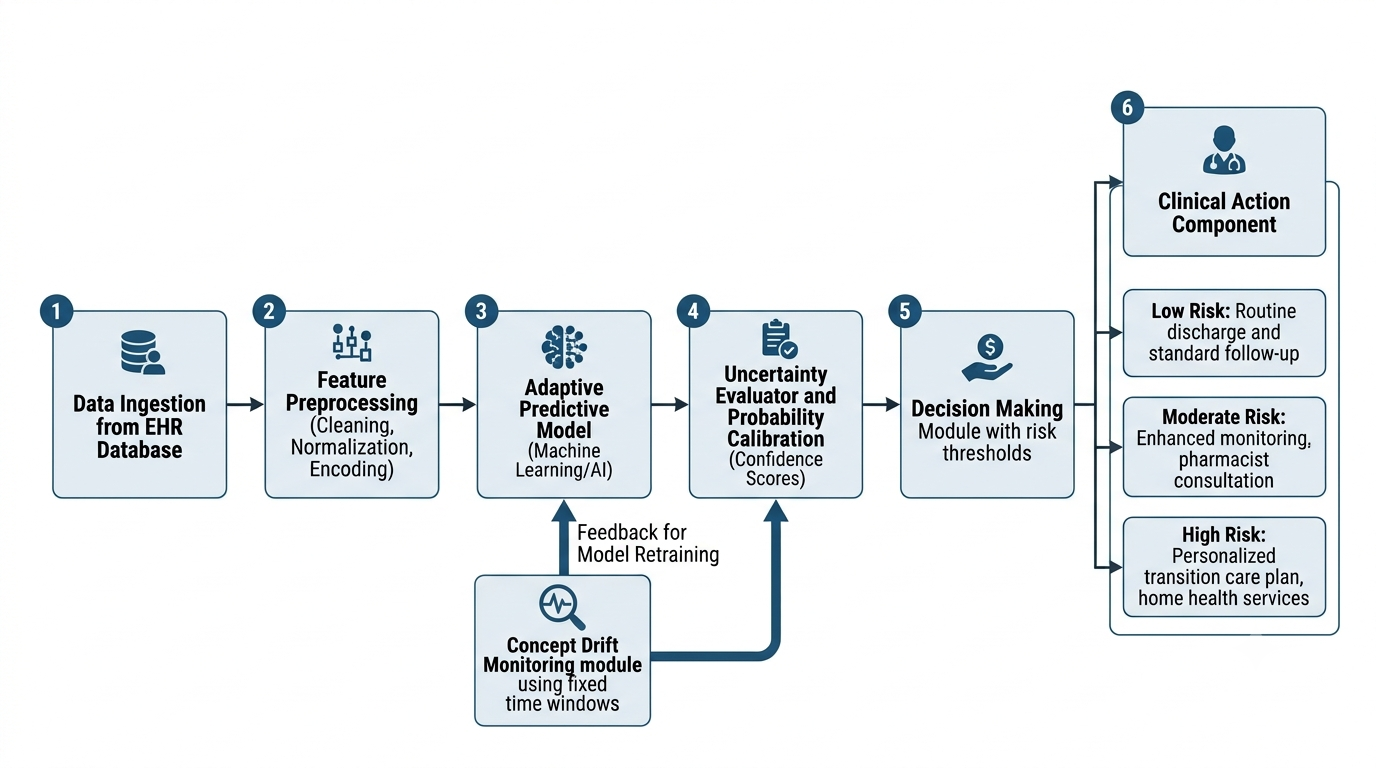
\includegraphics[width=0.6\textwidth]{arquitectura.png}
\caption{Arquitectura del sistema (seis módulos). El monitoreo de drift retroalimenta al modelo predictivo (reentrenamiento) y al evaluador de incertidumbre/calibración.}
\label{fig:arquitectura}
\end{figure}

El pipeline implementado sigue esta arquitectura módulo a módulo (\nb{01} a \nb{07}): cada vez que el drift dispara un reentrenamiento, el modelo (3) y su calibración (4) se reajustan sobre la ventana nueva.

% =====================================================================
\section{Modelos y Estrategia de Evaluación}
\label{sec:modelado}
% =====================================================================

La exploración de datos mostró evolución temporal en variables clave, lo que motivó variables de contexto en ventana deslizante y rezagadas/agregadas por periodo como candidatas de \emph{feature engineering} temporal. Antes de modelar, se auditó la preparación de datos con trece pruebas de fuga, dividiendo train/val/test en bloques estrictamente secuenciales (Sección~\ref{sec:restricciones}). La auditoría descartó las variables de contexto (actuaban como proxy del periodo, invalidando las curvas de drift) y corrigió un embargo de latencia insuficiente (\texttt{EMBARGO}: 850 $\to$ 2,000); todos los resultados se generaron después de esta corrección.

Se compararon dos enfoques tradicionales --\textbf{ElasticNet} (regresión logística regularizada) y \textbf{Random Forest} (ensamble de árboles)-- y uno más avanzado, \textbf{XGBoost} (\emph{gradient boosting}, mayor capacidad para interacciones no lineales entre diagnósticos, medicación y estancia). Cada modelo se ajusta con validación temporal (\texttt{TimeSeriesSplit}, 3 folds) sobre el 80\% inicial de la ventana de entrenamiento, y se calibra sobre el 20\% final entre Platt Scaling e Isotonic Regression \cite{platt1999} según cuál minimiza el Brier score.

\begin{table}[H]
\centering\small
\begin{tabular}{lccccccc}
\toprule
Modelo & ROC-AUC & PR-AUC & lift & Brier & BSS & pend. cal. & ECE \\
\midrule
ElasticNet & 0.652 & 0.213 & 1.87$\times$ & 0.098 & 0.031 & 1.014 & 0.023 \\
\textbf{RandomForest} & 0.664 & 0.215 & 1.89$\times$ & 0.098 & 0.030 & 1.017 & 0.027 \\
XGBoost & 0.653 & 0.192 & 1.69$\times$ & 0.099 & 0.020 & 0.774 & 0.028 \\
\bottomrule
\end{tabular}
\caption{Comparación de modelos, experimento E1 (estático, entrenado en bloques 1--2, evaluado sin reentrenar en bloques 3--10). Modelo principal en negrita.}
\label{tab:modelos}
\end{table}


Random Forest (en negrita) se selecciona como modelo principal por su mejor ROC-AUC y PR-AUC iniciales (Tabla~\ref{tab:modelos}).

% =====================================================================
\section{Monitoreo y Adaptación ante Data/Concept Drift}
\label{sec:drift}
% =====================================================================

Esta es la sección central del informe. Sigue el marco conceptual de la clase de \emph{Concept Drift} \cite{soriano2026}: un modelo se entrena sobre un concepto $P_{t_0}(X,y)$ y se aplica sobre datos futuros; existe drift cuando $P_{t_0}(X,y)\neq P_{t_1}(X,y)$ \cite{gama2014}. Se distingue \textbf{drift real} (cambia $P(y\mid X)$, la relación entre variables y etiqueta) de \textbf{drift virtual} (cambia $P(X)$ sin alterar esa relación); el primero exige reentrenar, el segundo puede degradar la calibración sin degradar necesariamente la discriminación.

\subsection{Metodología: ventanas fijas pseudo-temporales}

Al no disponer de fecha de admisión explícita, el dataset se ordena por \texttt{encounter\_id} (validado como proxy cronológico: el siguiente encuentro del mismo paciente registra hospitalizaciones previas en 84.9\% de los casos, vs.\ 47.4\% en orden inverso) y se divide en $N=10$ ventanas pseudo-temporales de tamaño equivalente (bloques 1--10, simulando periodos anuales).

\begin{itemize}[leftmargin=*]
    \item \textbf{Mapeo de degradación (E1, drift real):} el modelo se entrena una sola vez con los bloques 1--2 y se evalúa, sin reentrenar, en los bloques 3--10, cuantificando la pérdida de ROC-AUC/PR-AUC por drift temporal acumulado.
    \item \textbf{Monitoreo de distribución de \emph{features} (data drift básico):} para cada bloque $b>1$ se calcula el \emph{Population Stability Index} (PSI) \cite{siddiqi2006} y una prueba de hipótesis (Kolmogorov-Smirnov para variables numéricas, $\chi^2$ para categóricas, con corrección de Bonferroni por comparaciones múltiples) contra el bloque de referencia B1, sobre variables clínicas clave (uso de insulina, número de diagnósticos, procedimientos, urgencias, \texttt{race} para trazabilidad de equidad).
    \item \textbf{Protocolo de reentrenamiento fijo (E3):} ventana deslizante de tamaño $S$ bloques (se evaluó $S\in\{1,2,3,5\}$; $S=3$ es la configuración de referencia del plan de trabajo).
    \item \textbf{Ventana expansiva (E2):} el modelo se reentrena en cada bloque usando \emph{todo} el historial disponible hasta ese punto.
    \item \textbf{Disparador informado (E4):} el modelo parte del estático (B1--B2) y se reentrena \emph{solo} cuando se cumple alguno de tres criterios evaluados bloque a bloque: (a) caída de ROC-AUC $>0.03$ con intervalos de confianza al 95\% (bootstrap, $B=500$) sin solapar; (b) pendiente de calibración fuera de $[0.80,1.20]$; (c) PSI $>0.25$ en al menos 2 de 5 variables clave. Esto combina detección basada en tasa de error (a, b) y basada en distribución (c), los dos enfoques vistos en clase \cite{soriano2026}.
\end{itemize}

\paragraph{Nota de consistencia con el plan de trabajo original.} Una versión previa describía el disparador de E4 como ``el F1-score cae más de 0.05 puntos respecto a la referencia''; el proyecto \textbf{nunca calcula F1-score} (ver Métricas de Éxito: ROC-AUC/PR-AUC/Brier). El disparador realmente implementado es el criterio combinado AUC + calibración + PSI descrito arriba, más robusto que un único punto de corte.

\subsection{Resultados: distribución de \emph{features} (PSI)}

\begin{figure}[H]
\centering
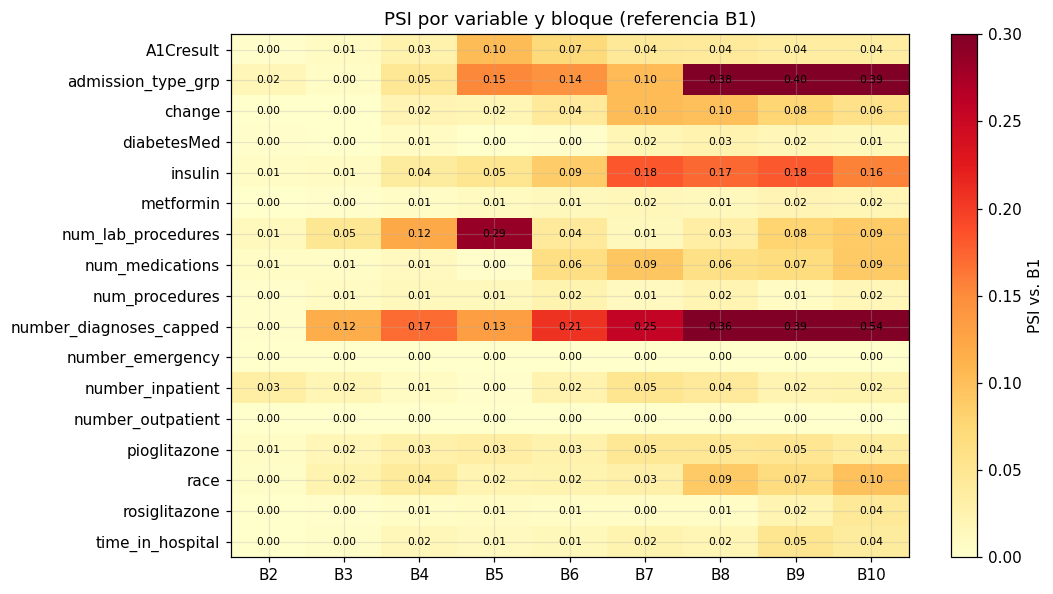
\includegraphics[width=0.5\textwidth]{../resultados/fig_psi_heatmap.png}
\caption{PSI por variable y bloque, respecto al bloque de referencia B1. Verde/amarillo = estable (PSI $<0.10$); rojo = alerta (PSI $>0.25$).}
\label{fig:psi-heatmap}
\end{figure}

\begin{table}[H]
\centering\small
\begin{minipage}{0.42\textwidth}
\centering
\begin{tabular}{lr}
\toprule
Estado PSI & \# (variable, bloque) \\
\midrule
estable & 131 \\
vigilar & 14 \\
ALERTA & 8 \\
\bottomrule
\end{tabular}
\end{minipage}%
\begin{minipage}{0.55\textwidth}
\centering
\begin{tabular}{clc}
\toprule
Bloque & Variable en ALERTA & PSI \\
\midrule
5 & num\_lab\_procedures & 0.286 \\
7 & number\_diagnoses\_capped & 0.255 \\
8 & admission\_type\_grp & 0.383 \\
8 & number\_diagnoses\_capped & 0.360 \\
9 & admission\_type\_grp & 0.400 \\
9 & number\_diagnoses\_capped & 0.395 \\
10 & number\_diagnoses\_capped & 0.540 \\
10 & admission\_type\_grp & 0.394 \\
\bottomrule
\end{tabular}
\end{minipage}
\caption{Izquierda: conteo de pares (variable, bloque) por estado de PSI respecto a B1 (131 estables, 14 en vigilancia, 8 en alerta, sobre 13 variables $\times$ 9 bloques evaluados). Derecha: alertas (PSI $>0.25$), concentradas en \texttt{number\_diagnoses\_capped} y \texttt{admission\_type\_grp} desde el bloque 7--8 en adelante.}
\label{tab:drift-resumen}
\end{table}


\subsection{Resultados: curva de degradación (E1) y comparación de estrategias}

\begin{figure}[H]
\centering
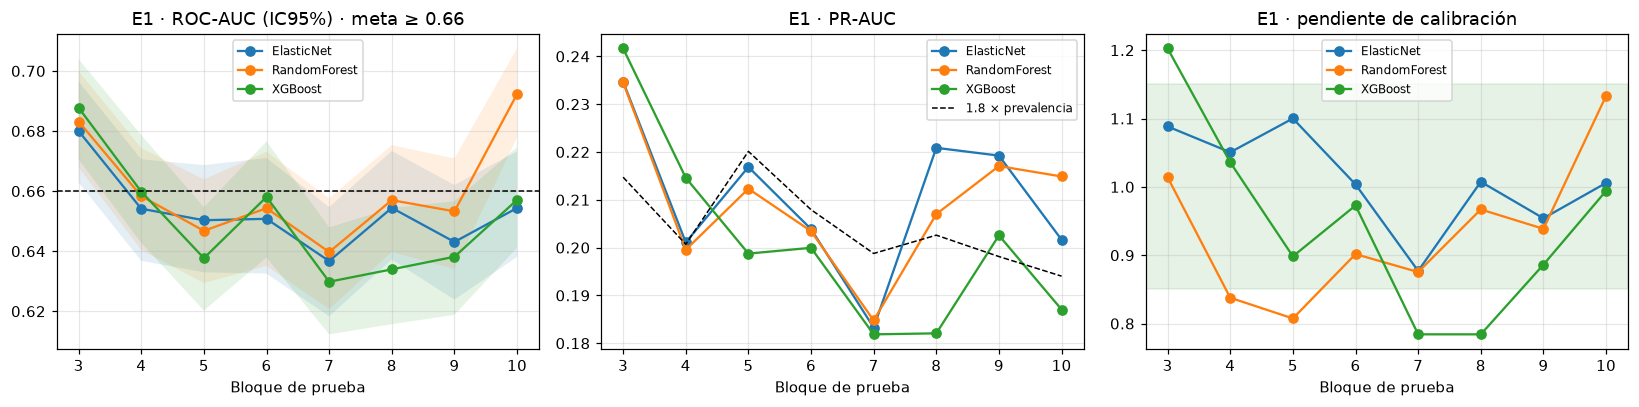
\includegraphics[width=0.5\textwidth]{../resultados/fig_E1_degradacion.png}
\caption{Curva de degradación del modelo estático (E1) por bloque de prueba: ROC-AUC, PR-AUC y pendiente de calibración, con intervalos de confianza al 95\%.}
\label{fig:e1-degradacion}
\end{figure}

{\small
\begin{longtable}{lcccc}
\toprule
Estrategia & ROC-AUC & PR-AUC & Brier & pend. cal. \\
\midrule
\endhead
\textbf{E3 deslizante S=3} & 0.680 & 0.226 & 0.095 & 1.123 \\
E2 expansiva & 0.676 & 0.223 & 0.095 & 1.075 \\
E3 deslizante S=2 & 0.676 & 0.222 & 0.095 & 1.053 \\
E4 disparador & 0.674 & 0.222 & 0.095 & 1.166 \\
E3 deslizante S=5 & 0.679 & 0.219 & 0.095 & 1.039 \\
E3 deslizante S=1 & 0.667 & 0.214 & 0.095 & 0.918 \\
E1 estático & 0.662 & 0.212 & 0.097 & 1.028 \\
\bottomrule
\caption{Comparación de estrategias de adaptación sobre bloques comunes (6--10). \textbf{E3 deslizante $S=3$} obtiene el mejor PR-AUC promedio entre E1/E2/E3 y se elige como estrategia desplegada para la capa de decisión --- coincide con la ventana de reentrenamiento de tamaño 3 propuesta originalmente en el plan de trabajo. E4 (disparador) se muestra por separado por ser condicional a los reentrenamientos que dispara (1 evento en el horizonte evaluado).}
\label{tab:estrategias}
\end{longtable}}

\textbf{E3 deslizante $S=3$} se elige como estrategia desplegada por su mejor PR-AUC promedio, coincidiendo con la ventana de reentrenamiento propuesta en el plan de trabajo.

\subsection{Granularidad del monitoreo}

Siguiendo la exploración pedida en el plan de trabajo (Fase 5), se repite el experimento E1 vs.\ E3 con $G\in\{5,10,15\}$ bloques: una granularidad más fina detecta el drift antes, a costa de ventanas más pequeñas y ruidosas. El reentrenamiento automático introduce un riesgo propio --degradar silenciosamente el modelo en producción-- que el esquema HITL y el \emph{shadow deployment} (Sección~\ref{sec:despliegue}) mitigan.

% =====================================================================
\section{Capa de Decisión y Caso de Negocio}
\label{sec:decision}
% =====================================================================

El umbral óptimo de intervención se deriva de la matriz de costos: $p^{*}=C_i/(C_r\cdot e)$. Los pacientes se categorizan en Bajo/Moderado/Alto Riesgo, con cupo máximo de 15\% en Alto Riesgo por bloque para evitar fatiga de alertas \cite{vandersijs2006}.

{\footnotesize
\setlength{\tabcolsep}{4pt}
\begin{longtable}{lrrrrr}
\toprule
Escenario & Modelo (3 cat.) & No interv. & Interv. a todos & Binario ($p\geq p^*$) & Ahorro vs.\ ref. \\
\midrule
\endhead
Base ($e=0.18$) & \$1,797,592 & \$1,822,600 & \$2,044,532 & \$1,807,089 & \$25,008 \\
Sensibilidad $e=0.12$ & \$1,806,584 & \$1,822,600 & \$2,153,888 & \$1,819,168 & \$16,016 \\
$e=0.18$ & \$1,797,592 & \$1,822,600 & \$2,044,532 & \$1,807,089 & \$25,008 \\
Sensibilidad $e=0.38$ & \$1,688,841 & \$1,822,600 & \$1,680,012 & \$1,600,345 & \$-8,829 \\
Ocupación $>$85\% & \$2,224,893 & \$2,278,250 & \$2,418,165 & \$2,230,297 & \$53,357 \\
\bottomrule
\caption{Costo esperado por cada 1,000 altas (US\$), promedio sobre bloques de decisión, bajo la estrategia adaptativa desplegada ($t_1,t_2$: umbrales Bajo/Moderado y Moderado/Alto).}
\label{tab:costos}
\end{longtable}}

\textbf{¿Vale la pena construir y mantener el monitoreo de drift, o basta con desplegar el modelo una vez?} Se compara la política \textbf{sin monitoreo} (umbrales fijados en bloques 1--2) contra \textbf{con monitoreo} (E3 $S=3$), proyectada a escala anual \supuesto{50,000 altas/año} \cite{strack2014}.

{\small
\begin{longtable}{lr}
\toprule
Concepto & Valor anual (US\$, 50,000 altas/año) \\
\midrule
\endhead
Costo esperado \textbf{sin} monitoreo (estático, umbral fijo) & \$90,268,164 \\
Costo esperado \textbf{con} monitoreo adaptativo (E3, $S=3$) & \$89,879,592 \\
\textbf{Ahorro bruto atribuible al monitoreo de drift} & \textbf{\$388,573} \\
Costo de mantenimiento del sistema (monitoreo + reentrenos) & \$2,934 \\
\textbf{Beneficio neto} & \textbf{\$385,639} \\
Retorno sobre la inversión (ROI) & 132x \\
\bottomrule
\caption{Caso de negocio anualizado (supuesto de escala: 50,000 altas/año).}
\label{tab:caso-negocio}
\end{longtable}}

El ahorro por cada 1,000 altas crece más de 16$\times$ entre el bloque 4 (\$924) y el bloque 10 (\$15,114): el valor del monitoreo aumenta con el tiempo, pues un modelo sin vigilancia se degrada progresivamente. El costo de mantenimiento (monitoreo + cómputo + reentrenos) se construyó de abajo hacia arriba, no se asumió gratuito \cite{sculley2015}.

% =====================================================================
\section{Auditoría de Equidad}
% =====================================================================

Se audita la paridad del sistema por grupo etario ($\geq$70 vs.\ $<$70 años) y por \texttt{race}, evaluando solo grupos con al menos 100 reingresos observados.

\begin{table}[H]
\centering\small
\begin{tabular}{llrrccc}
\toprule
Dimensión & Grupo & n & Reingresos & Tasa reingreso & Razón FNR & Cumple FNR \\
\midrule
grupo\_edad & $<$70 & 27,863 & 2,967 & 10.6\% & 1.00 & \ok \\
grupo\_edad & $\geq$70 & 23,636 & 2,880 & 12.2\% & 1.12 & \ok \\
race & AfricanAmerican & 9,186 & 1,018 & 11.1\% & 0.97 & \ok \\
race & Asian & 375 & 31 & 8.3\% & --- & n/e \\
race & Caucasian & 38,999 & 4,514 & 11.6\% & 1.00 & \ok \\
race & Desconocido & 1,096 & 102 & 9.3\% & 1.15 & \ok \\
race & Hispanic & 1,012 & 98 & 9.7\% & --- & n/e \\
race & Other & 831 & 84 & 10.1\% & --- & n/e \\
\bottomrule
\end{tabular}
\caption{Auditoría de equidad por grupo etario y raza. ``n/e'' = no evaluable ($<$100 reingresos). En la muestra evaluada, todos los grupos evaluables cumplen igualdad de oportunidad (razón de FNR). La razón de \emph{selección} a Alto Riesgo entre subgrupos (regla del 80\%) sí incumple (mínimo observado $\approx$0.38) por el mecanismo de cupo global --- ver discusión en la Sección de criterios no cumplidos.}
\label{tab:equidad}
\end{table}


El criterio de explicabilidad (top-3 factores SHAP, coincidentes con las variables monitoreadas por drift: insulina, diagnósticos, procedimientos y urgencias) se cumple en el 100\% de los casos, y la latencia (p95 $=79.5$ ms) cumple ampliamente la restricción de 2 segundos (Sección~\ref{sec:restricciones}).

% =====================================================================
\section{Resultados Consolidados y Criterios No Cumplidos}
\label{sec:resumen-criterios}
% =====================================================================

{\footnotesize
\begin{longtable}{p{1.5cm}p{3.2cm}p{3.0cm}p{4.2cm}c}
\toprule
\textbf{Dimensión} & \textbf{Métrica} & \textbf{Criterio} & \textbf{Resultado} & \textbf{Cumple} \\
\midrule
\endhead
Técnica & ROC-AUC & $\geq$ 0.66 & 0.673 (peor 0.646) & \ok \\
Técnica & PR-AUC / lift & $\geq$ 0.20 y $\geq$ 1.8$\times$ & 0.220 / 1.94$\times$ & \ok \\
Técnica & Brier & $\leq$ 0.095 & 0.0963 (BSS 0.044) & \fail \\
Técnica & Pendiente de calibración & [0.85, 1.15] & 1.05 (rango 0.78–1.44) & \ok \\
Técnica & Intercepto de calibración & [-0.15, 0.15] & -0.031 & \ok \\
Técnica & ECE & $\leq$ 0.02 & 0.0144 & \ok \\
Técnica & Latencia p95 & $<$ 1,000 ms & 111.3 ms & \ok \\
Decisión & Beneficio neto (DCA) & $\geq$ referencias en 0.05–0.30 & supera en 100\% del rango & \ok \\
Decisión & Costo esperado (base) & $<$ mín(referencias) & ahorro US\$25,008 / 1,000 altas & \ok \\
Decisión & Costo esperado (sensibilidad e) & $<$ mín(referencias) para e $\in$ {0.12, 0.18, 0.38} & 16,016 / 25,008 / -8,829 & \fail \\
Decisión & Impacto proyectado & $\geq$ 5\% & 3.8\% & \fail \\
Decisión & Tasa de Alto por bloque & $\leq$ 15\% & 15.0\% & \ok \\
Decisión & Tiempo de respuesta & $\geq$ 90\% contactados $\leq$ 7 días & N/A (despliegue) & --- \\
Social & Razón FNR edad ($\geq$70 vs $<$70) & [0.87, 1.15] & $\geq$70: 1.12 [1.09–1.14] & \ok \\
Social & Razón FNR raza (vs Caucasian) & [0.87, 1.15], $\geq$100 reingresos & AfricanAmerican: 0.97; Desconocido: 1.15 & \ok \\
Social & Razón de selección (80\%) & $\geq$ 0.80 & 0.38 & \fail \\
Social & Calibración por subgrupo & pendiente [0.8, 1.2], |int.| $\leq$ 0.2 & ver tabla de equidad & \ok \\
Social & Cobertura & $\geq$ 98\% & 100.0\% & \ok \\
Social & Incertidumbre Alta & $\leq$ 15\% & 37.6\% & \fail \\
Social & Reingreso en categoría Bajo & $<$ 8\% & 6.5\% & \ok \\
Social & Explicabilidad top-3 & 100\% & 100.0\% & \ok \\
Monitoreo & Reentrenamientos disparados (E4) & informativo & 1 & --- \\
Monitoreo & Variables con PSI > 0.25 (vs B1) & informativo & admission\_type\_grp, num\_lab\_procedures, number\_diagnoses\_capped & --- \\
\bottomrule
\caption{Tabla resumen de criterios de aprobación, estrategia desplegada (E3, $S=3$). 18 de 23 criterios cuantitativos se cumplen; los 5 restantes se discuten en el texto.}
\label{tab:resumen-criterios}
\end{longtable}}


De los 23 criterios evaluados, 18 se cumplen. Los 5 restantes --Brier, costo esperado en el escenario de sensibilidad más optimista ($e=0.38$), impacto proyectado, razón de selección (regla del 80\%) e incertidumbre alta-- comparten causa de fondo: el techo de discriminación del modelo (ROC-AUC $\approx0.67$), consistente con la literatura \cite{kansagara2011,emijohnson2025}. La razón de selección es la única brecha estructural --el cupo global de Alto Riesgo no garantiza paridad entre subgrupos con tasas base distintas \cite{chouldechova2017}-- y se documenta como limitación bloqueante de despliegue (Sección~\ref{sec:despliegue}).

% =====================================================================
\section{Propuesta de Despliegue y Gestión de Riesgos}
\label{sec:despliegue}
% =====================================================================

\subsection{Propuesta de despliegue}

Siguiendo el marco de opciones de despliegue visto en clase \cite{soriano2026}, se recomienda un despliegue por \textbf{microservicios en contenedor} (Docker) sobre \textbf{IaaS/PaaS} de nube --esta es la \textbf{arquitectura de implementación}--: el monitoreo de drift corre en \emph{batch} y el módulo predictivo sirve inferencia síncrona (SLA $<2$s \cite{nawaz2026}), por lo que conviene escalarlos por separado, con reproducibilidad garantizada por MLflow.

El \textbf{flujo de datos} sigue el ciclo EHR $\to$ ingesta/validación $\to$ preprocesamiento $\to$ inferencia $\to$ acción clínica, con cómputo periódico de PSI/KS/ROC-AUC (Sección~\ref{sec:drift}) que dispara el reentrenamiento (E4) con aprobación humana antes de reemplazar el modelo en producción (\emph{shadow deployment}) y registro auditable. La \textbf{frecuencia de actualización} no sigue calendario fijo: es condicional a la degradación bloque a bloque, consistente con que la deuda técnica de un sistema de ML vive en el ``glue code'' alrededor del modelo \cite{sculley2015}. La \textbf{autonomía} es parcial (HITL, Sección~\ref{sec:restricciones}): recomienda, el médico decide. Escalar implica \textbf{desafíos de costos} (cómputo por sede) e \textbf{integración} (EHR heterogéneos; migrar \texttt{encounter\_id} a fecha real).

\subsection{Riesgos identificados}

{\small
\begin{longtable}{p{2.9cm}p{4.7cm}p{4.9cm}}
\toprule
\textbf{Riesgo} & \textbf{Descripción} & \textbf{Mitigación} \\
\midrule
\endhead
Drift silencioso entre ciclos & Cambio abrupto degrada el modelo antes del siguiente chequeo. & Mayor frecuencia de monitoreo en periodos de alta variabilidad; alertas si PSI $>0.25$. \\
Fatiga de alertas clínicas & Exceso de Alto Riesgo reduce la atención a cada alerta \cite{vandersijs2006}. & Cupo de 15\% por bloque; monitorear tasa de \emph{override}. \\
Inequidad en la selección de Alto Riesgo & Razón de selección entre subgrupos por debajo de la regla del 80\%. & No desplegar sin resolver; evaluar cupos estratificados o post-procesamiento \cite{hardt2016}. \\
Fuga en cambios futuros / \texttt{encounter\_id} como proxy temporal & Nuevas variables pueden reintroducir fugas (Sección~\ref{sec:modelado}); el proxy solo es válido para este dataset histórico. & Repetir la batería de 13 pruebas de \texttt{auditoria\_leakage.csv} antes de integrar; migrar a fecha real de alta y revalidar embargo y ventanas. \\
\bottomrule
\end{longtable}}

% =====================================================================
\section{Conclusiones}
% =====================================================================

El sistema se diseñó, implementó y validó de punta a punta, cumpliendo el objetivo de mantener un desempeño confiable ante los cambios de los datos en el tiempo. La auditoría de fuga de información fue indispensable antes de confiar en las curvas de degradación reportadas. Las métricas cumplen la mayoría de los criterios \emph{a priori}; las excepciones (Brier, razón de selección) tienen explicación en literatura y mitigación propuesta. El caso de negocio muestra que el monitoreo de drift se paga solo frente a su costo de mantenimiento, entregando un sistema validado y un valor económico cuantificado.

% =====================================================================
\section*{Bibliografía}
\addcontentsline{toc}{section}{Bibliografía}
% =====================================================================

{\footnotesize
\begin{multicols}{2}
\begin{thebibliography}{99}

\bibitem{chouldechova2017} Chouldechova, A. (2017). Fair prediction with disparate impact: A study of bias in recidivism prediction instruments. \emph{Big Data}, 5(2), 153--163.

\bibitem{drincic2017} Drincic, A., Pfeffer, E., Luo, J., \& Goldner, W. S. (2017). The effect of diabetes case management and Diabetes Resource Nurse program on readmissions of patients with diabetes mellitus. \emph{Journal of Clinical \& Translational Endocrinology}, 8, 29--34.

\bibitem{emijohnson2025} Emi-Johnson, O., \& Nkrumah, K. (2025). Predicting hospital readmission risk with machine learning: benchmarks on the Diabetes 130-US hospitals dataset.

\bibitem{gama2014} Gama, J., Žliobaitė, I., Bifet, A., Pechenizkiy, M., \& Bouchachia, A. (2014). A survey on concept drift adaptation. \emph{ACM Computing Surveys}, 46(4), 1--37.

\bibitem{ghabowen2024} Ghabowen, I., et al. (2024). Cost of hospital readmissions attributable to diabetes.

\bibitem{hardt2016} Hardt, M., Price, E., \& Srebro, N. (2016). Equality of opportunity in supervised learning. \emph{Advances in Neural Information Processing Systems (NeurIPS)}, 29.

\bibitem{kansagara2011} Kansagara, D., et al. (2011). Risk prediction models for hospital readmission: a systematic review. \emph{JAMA}, 306(15), 1688--1698.

\bibitem{leppin2014} Leppin, A. L., et al. (2014). Preventing 30-day hospital readmissions: a systematic review and meta-analysis of randomized trials. \emph{JAMA Internal Medicine}, 174(7), 1095--1107.

\bibitem{nawaz2026} Nawaz. (2026). \emph{How to instrument clinical decision support system response times}. OneUptime.

\bibitem{platt1999} Platt, J. (1999). Probabilistic outputs for support vector machines and comparisons to regularized likelihood methods. \emph{Advances in Large Margin Classifiers}, 10(3), 61--74.

\bibitem{saito2015} Saito, T., \& Rehmsmeier, M. (2015). The precision-recall plot is more informative than the ROC plot when evaluating binary classifiers on imbalanced datasets. \emph{PLOS ONE}, 10(3).

\bibitem{salim2026} Salim, \& Ibrahim. (2026). Calibrated risk prediction for hospital readmission with nested cross-validation. \emph{Research Square} (preprint).

\bibitem{sculley2015} Sculley, D., Holt, G., Golovin, D., Davydov, E., Phillips, T., Ebner, D., Chaudhary, V., Young, M., Crespo, J.-F., \& Dennison, D. (2015). Hidden technical debt in machine learning systems. \emph{Advances in Neural Information Processing Systems (NeurIPS)}, 28.

\bibitem{siddiqi2006} Siddiqi, N. (2006). \emph{Credit Risk Scorecards: Developing and Implementing Intelligent Credit Scoring}. Wiley.

\bibitem{soriano2026} Soriano-Vargas, A. (2026). \emph{Concept Drift} [Diapositivas de clase, Planificación y Toma de Decisiones en IA]. UTEC.

\bibitem{strack2014} Strack, B., DeShazo, J. P., Gennings, C., Olmo, J. L., Ventura, S., Cios, K. J., \& Clore, J. N. (2014). Impact of HbA1c measurement on hospital readmission rates: analysis of 70,000 clinical database patient records. \emph{BioMed Research International}, 2014.

\bibitem{vandersijs2006} van der Sijs, H., et al. (2006). Overriding of drug safety alerts in computerized physician order entry. \emph{Journal of the American Medical Informatics Association}, 13(2), 138--147.

\bibitem{vanwalraven2011} van Walraven, C., Bennett, C., Jennings, A., Austin, P. C., \& Forster, A. J. (2011). Proportion of hospital readmissions deemed avoidable: a systematic review. \emph{Canadian Medical Association Journal}, 183(7), E391--E402.

\bibitem{vickers2006} Vickers, A. J., \& Elkin, E. B. (2006). Decision curve analysis: a novel method for evaluating prediction models. \emph{Medical Decision Making}, 26(6), 565--574.

\end{thebibliography}
\end{multicols}}

\end{document}
